To determine under which conditions a Beta regression model can well approximate the Rank-Ordered Logit model in the estimation of the ability parameters in a multi-competitor game context, a model-based simulation study was conducted. We simulated data according to Algorithm \ref{alg:sim}: \\
\\
\begin{algorithm}[H]
  \SetAlgoLined
  \KwIn{\begin{itemize}
  \item number of games $n\_games$;
  \item total number of competitors $n\_comp$;
  \item number of entrants per game $n\_per\_game$;
  \item standard deviation of ability parameters $\sigma$.
\end{itemize}}
  \KwOut{ranking of competitors in $n\_games$}
  \textbf{Step 1.} A vector of abilities $\boldsymbol{\theta}$ is created, by randomly sampling $n\_comp$ values from a $Normal(0,\sigma)$ distribution; \\
  \For{each of $n\_games$}{
    \textbf{Step 2.} Competitors indices $comp\_ids$ are created by randomly sampling  $n\_per\_game$ values without replacement from the interval (1,$n\_comp$);\\
    \textbf{Step 3.} A vector $Y$ of $n\_per\_game$ performance values is generated from a Gumbel($\boldsymbol{\theta}[comp\_ids])$ distribution\;
    \textbf{Step 4.} $Y$ is sorted in descending order;\\
    \textbf{Step 5.} The indices of competitors associated to each performance in the ordered $Y$ generated in Step 4 provides the ranking of competitors in the game;
  }
  \textbf{Step 6.} Rankings of competitors from each game are combined together; 
  \caption{ROL-based simulation of rankings of competitors in multiple games}\label{alg:sim}
\end{algorithm}
\newpage
\noindent Factors that were changed in the simulation are: total number of competitors, number of entrants per game, number of games and standard deviation of abilities. A summary of the different levels used for each of them is given in Table \ref{tab}.
\begin{table}[h]
\centering
\begin{tabular}{l|l}
   Factor  & Levels \\
\hline
Total number of competitors & $n\_comp$= 15, 50, 250, 500\\
Number of entrants per game & $n\_per\_game$ = 2, 8, 20, 40 \\
Number of games & $n\_game$ = 20, 50, 250, 1250\\
Standard deviation of abilities & $\sigma$ = 0.1, 1, 10
\end{tabular}
\caption{Different levels used for each factor in the simulations.}
\label{tab}
\end{table}
\\
\begin{itemize}
  \item \underline{Total number of competitors} \\ The first  level  ($n\_comp$=15) represents the threshold mentioned by  Alvo et Philip (2014) referring to the point after which the ROL model becomes too computationally intense, the second one ($n\_comp$=50) represents the number of competitors typical of real world competitions such as ski races, and the remaining  two levels, ($n\_comp$=250 and $n\_comp$=500) aim to simulate contexts where the number of potential competitors is considerably large, as is the case in online games. 
 \item \underline{Number of entrants per game}\\ The tested levels for this factor replicate the number of competitors competing against each others in different sports. For example, $n\_per\_game$ =2 simulate the outcome of a head-to-head competition such as a tennis match. The second one ($n\_per\_game$ =8)  reassemble an athletics competition; the third one ($n\_per\_game$= 20) approximate the number of entrants in a Formula One race and the last level ($n\_per\_game$= 40) the number of cars competing in NASCAR races. 
  \item \underline{Number of games}\\ 
  This factor constitutes the sample size as each game represents one observation. The uncertainty around the estimate of the ability parameters for both models is expected to decrease for increasing number of games.
  \item \underline{Standard deviation of abilities}\\
 Different variances were chosen to imitate different  scenarios ranging from situations in which players are characterised basically by the the same ability ($\sigma$=0.1) to context where they significantly differ ($\sigma$=10), as is often the case in sports where the same competitors are winning every time. 
\end{itemize}
For each combination of these levels 1000 dataset were generated.\\
The Rank-Ordered Logit model and the Beta regression one were then fitted to each dataset. Parameters were estimated using a Bayesian approach through the use of Stan statistical modeling language (\cite{stan2018stan}). Bayesian estimation methods were chosen because they better adapt to model ranking data. Indeed, as stressed by \cite{guiver2009bayesian}, maximum likelihood estimation algorithms for Plackett-Luce model may not reach convergence and lead to over-fitting in presence of sparse data.\\
Performance of both models was evaluated by looking at the mean squared error between the known ability parameters and the estimated ones. The estimates were provided by the mean of the posterior distributions of the parameters and 95\% credible intervals were also computed  to give a measure of the uncertainty around them. An example of a graphical representation of how the comparison between the two models could look like is given in Figure \ref{fig: ROL, Beta and true ability parameters for five competitors}.\footnote{The example dataset used for this representation simulated 5 competitors competing against each other in 100 games with a standard deviation for the ability parameters equals to 1.}\\
\begin{figure}[h]
\centering
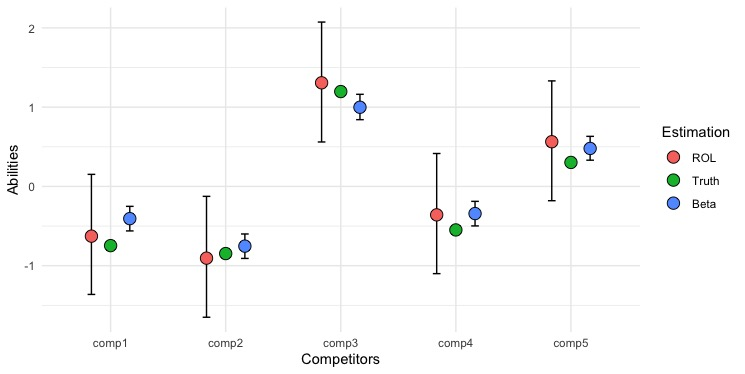
\includegraphics[scale=0.5]{images/Rplot01.jpeg}
\caption{True abilities and ROL and Beta estimated ones with 95\% credible intervals for five competitors}
\label{fig: ROL, Beta and true ability parameters for five competitors}
\end{figure}
\\
The analysis was conducted using package “CmdStanR” (\cite{gabry2021cmdstanr}) in R studio version 4.2.1 (\cite{posit2023rstudio}).
